\section{Results}
\label{sec:results}

\subsection{RQ1: random versus chronological evaluation}
\label{sec:res-split}
\Cref{tab:split} trains the same classifier on 30\% of each dataset, either a stratified random 30\% or the first
30\% in time, and scores it closed-world on the rest, as the papers that report near-perfect results do.

On a random split, the classifier reproduces the familiar numbers: 99.8\% accuracy on CIC-IDS2017 and 98.5\% on
CSE-CIC-IDS2018. Chronologically, accuracy falls to 72.6\% and 85.0\%, and macro-F1 collapses from 0.761 to 0.125
and from 0.692 to 0.071, because eleven and seven of the test-period classes never occur in training. Accuracy
hides most of the collapse, because the majority of flows are benign and benign traffic is still recognised.
Even on the random split, macro-F1 is far below accuracy: rare classes such as SQL injection or infiltration, with a
handful of flows, are not learned, and accuracy does not show it.

UNSW-NB15 behaves differently. Every class occurs on its first capture day, so the chronological split creates no
new classes, and accuracy changes little (97.8\% to 96.4\%). Its low macro-F1 under both splits reflects the
known overlap of several of its attack categories; DoS and Exploits, for example, are hard to separate even when
both are in training. This is why we hold four classes out of its training period in the remaining experiments.

\begin{table}[t]
\centering
\caption{The same classifier on a random and a chronological 30/70 split (closed-world scoring, no \unk{}).
Random split: mean of three seeds (standard deviation $\le 0.018$).}
\label{tab:split}
\small
\IfFileExists{\results{split_check_paper.tex}}{%
\CatchFileDef{\splitrows}{\results{split_check_paper.tex}}{}%
\begin{tabular}{@{}lccccc@{}}
\toprule
 & \multicolumn{2}{c}{Random split} & \multicolumn{2}{c}{Chronological split} & Test classes \\
Dataset & Accuracy & Macro-F1 & Accuracy & Macro-F1 & unseen in training \\
\midrule
\splitrows
\bottomrule
\end{tabular}}{\TBD{split table not generated yet}}
\end{table}

The answer to RQ1 is that random-split accuracy says little about a deployed detector. In the remaining
experiments every method is evaluated chronologically and open-world, and a method that cannot name a new attack
can at least reject it as \unk{}.

\subsection{RQ2: main comparison}
\label{sec:res-main}
\resulttable[p]{CIC17_main_b010_paper.tex}{CIC-IDS2017 (development dataset), label budget 10\%, delay 1 window, five seeds.}{tab:cic17}
\resulttable[p]{IDS18_main_b010_paper.tex}{CSE-CIC-IDS2018 (held out), label budget 10\%, delay 1 window, five seeds.}{tab:ids18}
\resulttable[p]{UNSW_main_b010_paper.tex}{UNSW-NB15 (held out; DoS, Reconnaissance, Shellcode and Worms removed from training), label budget 10\%, delay 1 window, five seeds.}{tab:unsw}

\begin{figure}[p]
\centering
\IfFileExists{\results{fig_ow_f1_over_time_CIC17.pdf}}{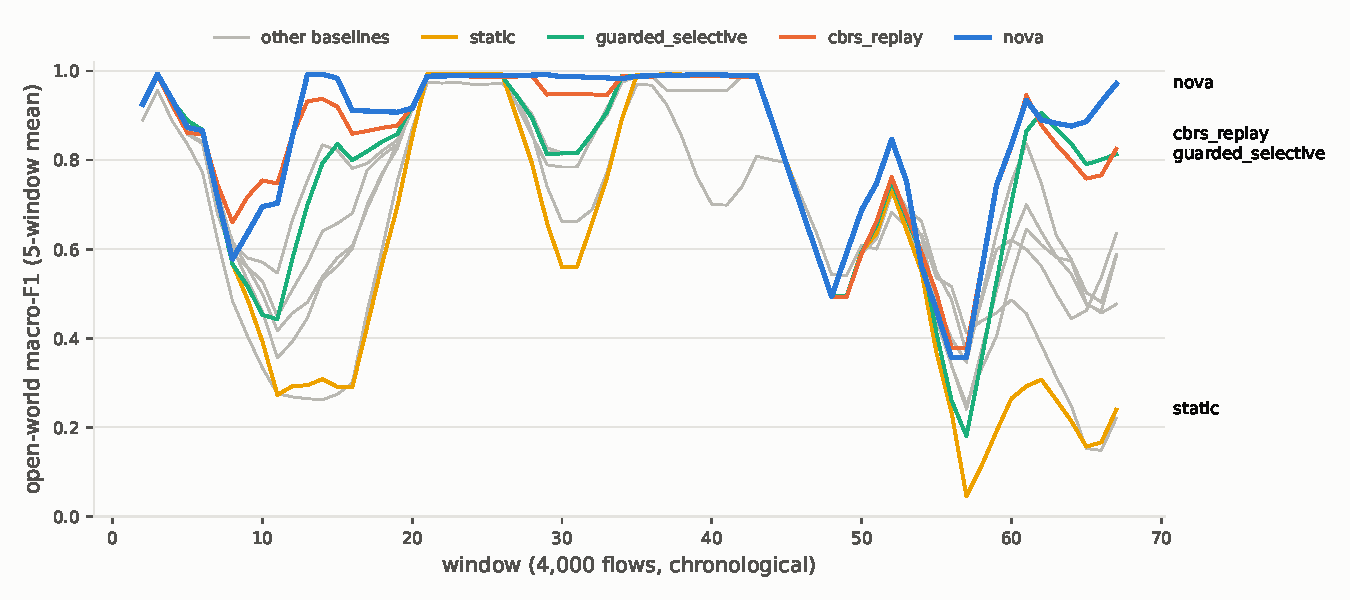
\includegraphics[width=0.78\textwidth]{fig_ow_f1_over_time_CIC17.pdf}}{\TBD{figure}}\\[2pt]
{\small (a) CIC-IDS2017}\\[6pt]
\IfFileExists{\results{fig_ow_f1_over_time_IDS18.pdf}}{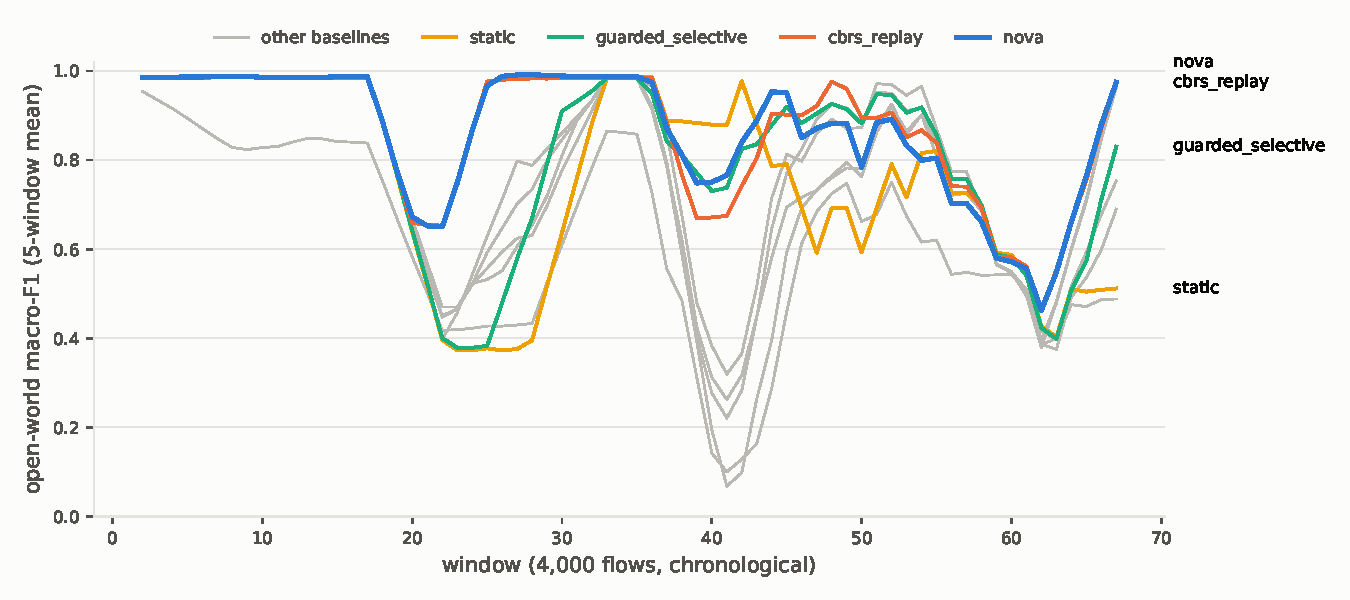
\includegraphics[width=0.78\textwidth]{fig_ow_f1_over_time_IDS18.pdf}}{\TBD{figure}}\\[2pt]
{\small (b) CSE-CIC-IDS2018}\\[6pt]
\IfFileExists{\results{fig_ow_f1_over_time_UNSW.pdf}}{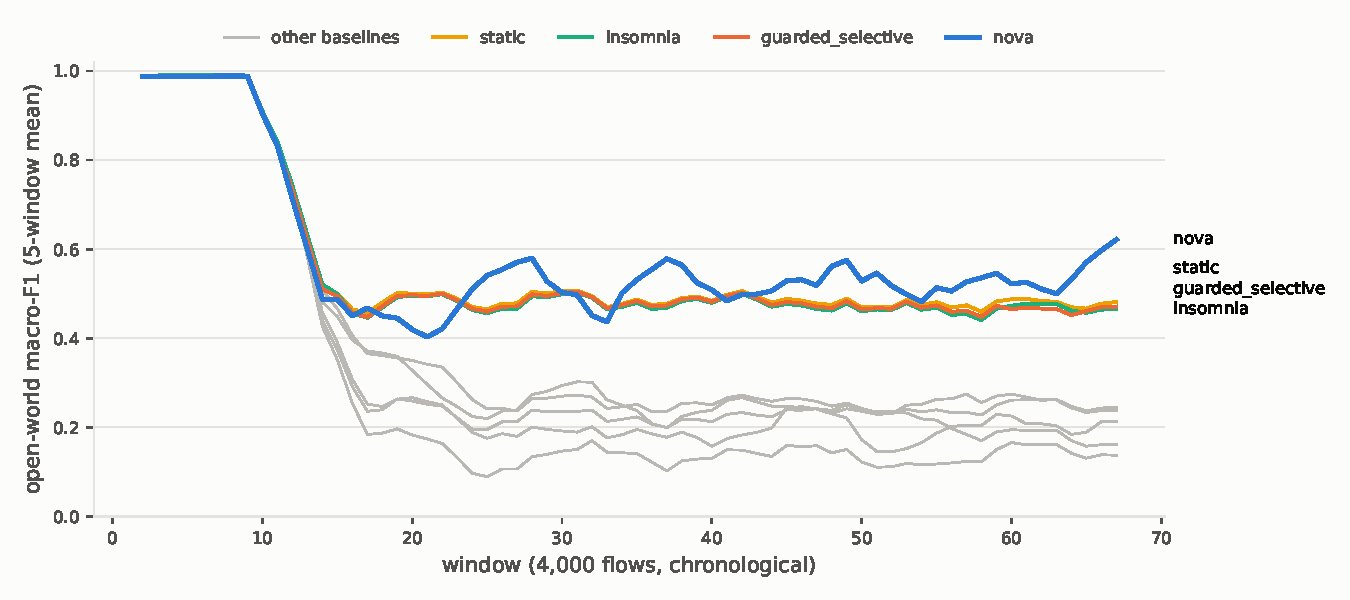
\includegraphics[width=0.78\textwidth]{fig_ow_f1_over_time_UNSW.pdf}}{\TBD{figure}}\\[2pt]
{\small (c) UNSW-NB15}
\caption{Open-world macro-F1 per window (mean of five seeds, 5-window moving average). \nova{}, the strongest
baselines and the static model are in colour; the remaining baselines are grey.}
\label{fig:time}
\end{figure}

\textbf{CIC-IDS2017} (\cref{tab:cic17}, \cref{fig:time}a). \nova{} and CBRS replay tie on OW-F1 (0.752 against
0.755). \nova{} has the higher AUT (0.860 against 0.837) and is better in 52 of the 70 windows, but the per-window
difference is within the bootstrap uncertainty ($+2.2$ points, 95\% CI $[-0.3, +4.6]$, \cref{tab:boot}). \nova{}
also varies more across seeds (0.721 to 0.776, against 0.752 to 0.757 for CBRS replay); in the two lower seeds it
names DoS GoldenEye and SQL injection less well. \nova{} is significantly ahead of every other method, by 7.0 to
23.1 points. CBRS detects slightly more attacks (detection F1 0.863 against 0.858, unknown AUROC 0.884 against
0.868), but \nova{} flags significantly fewer benign flows (2.8\% against 4.5\% pooled; per-window difference
$-4.2$ points, CI $[-9.0, -0.4]$): it sends 38\% fewer benign flows to the analyst.
The static model, which never sees a label, ends at 0.316 because every attack class in the stream is new to it.
\Cref{fig:time}a shows the shape of the stream: each attack day opens with a dip, while the new class is unknown
and partly missed, and the adaptive methods recover once labels arrive; \nova{} is on or near the top after most dips.

\textbf{CSE-CIC-IDS2018} (\cref{tab:ids18}, \cref{fig:time}b). \nova{} and CBRS replay tie on OW-F1 (0.738 against
0.730) and AUT (0.867 against 0.870). \nova{} is better in 50 of the 70 windows, but CBRS is ahead by three points
on average over the last 24 windows, the per-window difference is close to zero ($-0.4$, CI $[-2.3, +1.4]$), and
\nova{} varies more across seeds (0.655 to 0.793). On the other metrics \nova{} is ahead: detection F1 0.803 against
0.784, a significantly lower false-positive rate (3.2\% against 4.7\%; CI $[-5.5, -0.4]$), and maximum forgetting
0.008 against 0.032. Guarded selective retraining has the lowest false-positive rate on this dataset (2.7\%), but
it detects far fewer attacks (detection F1 0.592).

\textbf{UNSW-NB15} (\cref{tab:unsw}, \cref{fig:time}c). Here most adaptive methods end \emph{below} the static
model (0.499): CBRS replay reaches 0.326, continual replay 0.352 and uncertainty sampling 0.241. The per-flow
predictions show why. These methods learn Exploits and Fuzzers, but every flow of these classes is then rejected
as \unk{} (\cref{sec:res-perclass}). The open-world thresholds were calibrated on the January reference set, and
the February traffic of the same classes lies outside them. Classes that the model has learned are no longer
credited for \unk{}, so the rejections count as errors.

\nova{} recalibrates each learned class on recent labelled flows that it did not train on (the calibration store)
and reaches 0.511 OW-F1 and 0.596 AUT. This is significantly ahead of every replay-based method ($+19.6$ to
$+29.4$ points) and of guarded selective retraining ($+3.4$, CI $[+0.5, +5.8]$), and level with the static model
($+2.7$, CI $[-0.0, +4.9]$). It also has the highest detection F1 (0.858) and the lowest false-positive rate
(6.7\% against 7.5--19.0\%). Every method flags all UNSW-NB15 attack flows (detection recall 1.0), so on this
dataset the methods differ in false positives and in naming the attack class, not in missed attacks.

\textbf{Self-training.} INSOMNIA, which labels half of each window with its own nearest-centroid estimator, has
the highest false-positive rate on both CIC datasets (12.4\% and 25.8\%) and the largest forgetting on
CSE-CIC-IDS2018 (0.142). Its estimator can only assign classes that existed at training time, so flows of new
attacks are fed back into training under wrong labels.

\begin{table}[t]
\centering
\caption{Per-window difference \nova{} minus method, in points, with 95\% moving-block bootstrap intervals. OW-F1 at
budgets 10\% and 1\% (positive: \nova{} better), and false-positive rate at 10\% (negative: \nova{} flags fewer
benign flows). Intervals that exclude zero are significant.}
\label{tab:boot}
\small
\setlength{\tabcolsep}{3pt}
\loadrows{\bootA}{bootstrap_paper.tex}{4}\loadrows{\bootB}{bootstrap_b001_paper.tex}{4}%
\loadrows{\bootC}{bootstrap_fpr_paper.tex}{4}%
\resizebox{\textwidth}{!}{%
\begin{tabular}{@{}lccc@{}}
\toprule
Method & CIC-IDS2017 & CSE-CIC-IDS2018 & UNSW-NB15 \\
\midrule
\multicolumn{4}{@{}l}{\emph{OW-F1, budget 10\%}} \\
\bootA
\midrule
\multicolumn{4}{@{}l}{\emph{OW-F1, budget 1\%}} \\
\bootB
\midrule
\multicolumn{4}{@{}l}{\emph{False-positive rate, budget 10\%}} \\
\bootC
\bottomrule
\end{tabular}}
\end{table}

\textbf{Answer to RQ2.} At a 10\% budget, \nova{} ties with the strongest baseline, CBRS replay, on both CIC
datasets (stream-level differences of $-0.3$ and $+0.8$ points; per-window differences within the bootstrap
uncertainty, \cref{tab:boot}) and has the highest OW-F1 on UNSW-NB15. What is robust is the false-positive rate: \nova{} flags significantly
fewer benign flows than CBRS replay on all three datasets. The largest accuracy gap, on UNSW-NB15, comes from
recalibration; \cref{sec:res-ablation} confirms this.

\subsection{RQ3: ten times fewer labels}
\label{sec:res-budget}
\Cref{tab:budget} repeats the comparison with 1\% of each window labelled (40 flows per window) and an unchanged
configuration. The two label-free methods are omitted, because their results do not depend on the budget.

\begin{table}[t]
\centering
\caption{Label budget 1\%: OW macro-F1 and false-positive rate (\%), mean over five seeds; best per column in
bold.}
\label{tab:budget}
\small
\setlength{\tabcolsep}{4pt}
\IfFileExists{\results{budget_b001_paper.tex}}{%
\CatchFileDef{\budgetrows}{\results{budget_b001_paper.tex}}{}%
\begin{tabular}{@{}lcccccc@{}}
\toprule
\budgetrows
\bottomrule
\end{tabular}}{\TBD{budget table not generated yet}}
\end{table}

On CIC-IDS2017, where the two methods tie at 10\%, \nova{} leads CBRS replay at 1\% by 8.5 OW-F1 points (0.651
against 0.566) and 5.7 AUT points (0.818 against 0.761). \nova{} loses 0.101 OW-F1 when the budget shrinks
tenfold, CBRS replay 0.189. Unknown AUROC stays at 0.869 for \nova{} but falls to 0.787 for CBRS replay. The
per-window lead over CBRS replay is significant ($+5.7$ points, CI $[+1.4, +10.2]$). On CSE-CIC-IDS2018, \nova{}
is slightly ahead at 1\% (0.559 against 0.541; AUT 0.825 against 0.808), but the interval includes zero ($+1.5$,
CI $[-0.0, +4.7]$).

On UNSW-NB15, \nova{} is behind at 1\%: 0.470 against 0.501 for periodic retraining, significantly so per window
($-5.0$, CI $[-10.3, -0.9]$), and 0.478 for continual replay and guarded selective retraining (not significant). The per-class results show that this lead comes from \emph{not} learning. With
40 labels per window, periodic retraining never collects the five labels per class it needs to learn the four
held-out classes: in all five seeds its last model knows none of them. It keeps rejecting these classes as \unk{}, which the metric credits in full
(per-class F1 0.90 to 1.00), while it scores 0 on Exploits and Fuzzers, like the static model.

\nova{} spends its labels on novel flows, so it does learn DoS and Reconnaissance. In UNSW-NB15, however, these
overlap heavily with Exploits; in the first seed, 38\% of the DoS flows scored after DoS was learned are labelled
Exploits. A class that is learned but confused scores lower than a class that stays \unk{}. At the same time,
\nova{} has by far the lowest false-positive rate (10.7\% against 16.2--18.5\%) and the highest detection F1 (0.793
against at most 0.715).

\textbf{Answer to RQ3.} When labels are scarce, \nova{} pulls ahead on both CIC datasets, significantly on
CIC-IDS2017; the ablation of
\cref{sec:res-ablation} suggests that the query, which mainly improves unknown detection, contributes to this,
although we did not repeat the ablation at 1\%. The UNSW-NB15 result is a limit of open-world scoring, not of the query: open-world macro-F1 rewards
leaving an inseparable class unknown over learning it. Operators who prefer the second outcome should read
OW-F1 together with per-class results.

\subsection{Decomposing the open-world score}
\label{sec:res-decomp}
Because open-world macro-F1 merges two different outcomes, ``the class is unknown and rejected'' and ``the class
is known and named correctly'', \cref{tab:decomp} reports them separately from the per-flow predictions. Each flow
is either of a class known to the model that scored it, or of a class unknown to it. On known-class flows we
report macro-F1 (with \unk{} counted as an error), the share wrongly rejected as \unk{}, and the share of known
\emph{attack} flows named with their correct class. On unknown-class flows we report the share rejected as \unk{}
(unknown recall). Among all \unk{} decisions we report the share that are indeed of an unknown class (unknown
precision).

\begin{table}[t]
\centering
\caption{Open-world outcomes separated (mean over five seeds). Known: flows of classes the deployed model knows;
unknown: flows of classes it does not know.}
\label{tab:decomp}
\small
\setlength{\tabcolsep}{4pt}
\loadrows{\decA}{owparts_CIC17_b010_paper.tex}{6}\loadrows{\decB}{owparts_IDS18_b010_paper.tex}{6}%
\loadrows{\decC}{owparts_UNSW_b010_paper.tex}{6}\loadrows{\decD}{owparts_UNSW_b001_paper.tex}{6}%
\resizebox{\textwidth}{!}{%
\begin{tabular}{@{}lccccc@{}}
\toprule
 & \multicolumn{3}{c}{Known-class flows} & \multicolumn{2}{c}{Unknown-class flows} \\
\cmidrule(lr){2-4}\cmidrule(l){5-6}
Method & Macro-F1 & Falsely rejected (\%) & Attacks named correctly & Recall & Precision \\
\midrule
\multicolumn{6}{@{}l}{\emph{CIC-IDS2017, budget 10\%}} \\
\decA
\midrule
\multicolumn{6}{@{}l}{\emph{CSE-CIC-IDS2018, budget 10\%}} \\
\decB
\midrule
\multicolumn{6}{@{}l}{\emph{UNSW-NB15, budget 10\%}} \\
\decC
\midrule
\multicolumn{6}{@{}l}{\emph{UNSW-NB15, budget 1\%}} \\
\decD
\bottomrule
\end{tabular}}
\end{table}

The decomposition separates the methods more clearly than OW-F1 does. On UNSW-NB15 at 1\%, periodic retraining,
which won on OW-F1, reaches a known-class macro-F1 of only 0.150 and names 6\% of known attack flows correctly;
\nova{} reaches 0.390 and 62\%. Its OW-F1 lead therefore comes entirely from the \unk{} credit for classes it
never learns. At 10\%, \nova{}'s known-class macro-F1 on UNSW-NB15 is 0.505 against at most 0.165, and it wrongly
rejects 5.5\% of known flows against 13.4--31.1\% for the other methods, which is the stale-threshold failure in
numbers.

The decomposition also shows where \nova{} is weaker. On CSE-CIC-IDS2018, CBRS replay has the higher known-class
macro-F1 (0.781 against 0.744) and rejects more unknown flows (recall 0.668 against 0.554). \nova{}'s advantage there
is the precision of its \unk{} decisions (0.415 against 0.317), i.e.\ fewer benign or known flows sent to the
analyst as unknown. On CIC-IDS2017, \nova{} has the higher known-class macro-F1 (0.782 against 0.574) and attack
identification (0.755 against 0.667), while CBRS again rejects more unknown flows (0.614 against 0.438). Unknown
precision is low for every method on UNSW-NB15 (at most 0.10), because unknown-class flows are rare there and
most \unk{} decisions concern drifted benign traffic.

\subsection{RQ4: which components matter}
\label{sec:res-ablation}
\Cref{tab:ablation} removes one component at a time on all three datasets, and \cref{tab:ablation-ci} gives the
per-window differences with block-bootstrap intervals. The CIC-IDS2017 ablation was part of the development. The
two held-out ablations were run after the main results, with the method unchanged. The ablations use three seeds,
and full \nova{} is taken from the same three seeds of the main comparison.

The two views can disagree. Stream-level OW-F1 gives every class the same weight, so a class with a few dozen
flows counts as much as all benign traffic. The per-window difference gives every window the same weight, so a
component that matters only for a short-lived class barely moves it.

\begin{table}[t]
\centering
\caption{Ablation: stream-level OW macro-F1 (change against full \nova{} in points) and false-positive rate (\%)
with one component removed; budget 10\%, mean over three seeds. Full \nova{} is the mean over the same three seeds,
so it can differ slightly from \cref{tab:cic17,tab:ids18,tab:unsw}.}
\label{tab:ablation}
\small
\setlength{\tabcolsep}{4pt}
\IfFileExists{\results{ablation_all_paper.tex}}{%
\CatchFileDef{\ablrows}{\results{ablation_all_paper.tex}}{}%
\resizebox{\textwidth}{!}{%
\begin{tabular}{@{}lcccccc@{}}
\toprule
 & \multicolumn{2}{c}{CIC-IDS2017} & \multicolumn{2}{c}{CSE-CIC-IDS2018} & \multicolumn{2}{c}{UNSW-NB15} \\
Variant & OW-F1 & FPR & OW-F1 & FPR & OW-F1 & FPR \\
\midrule
\ablrows
\bottomrule
\end{tabular}}}{\TBD{ablation table not generated yet}}
\end{table}

\begin{table}[t]
\centering
\caption{Ablation, per window: mean difference ablated minus full \nova{} over the 70 windows (points, both
averaged over the same three seeds), with 95\% moving-block bootstrap intervals. Negative OW-F1 and positive FPR
differences mean that the component helps.}
\label{tab:ablation-ci}
\small
\setlength{\tabcolsep}{4pt}
\loadrows{\ablciA}{bootstrap_ablation_paper.tex}{4}%
\loadrows{\ablciB}{bootstrap_ablation_fpr_paper.tex}{4}%
\resizebox{\textwidth}{!}{%
\begin{tabular}{@{}lccc@{}}
\toprule
Variant & CIC-IDS2017 & CSE-CIC-IDS2018 & UNSW-NB15 \\
\midrule
\multicolumn{4}{@{}l}{\emph{OW macro-F1}} \\
\ablciA
\midrule
\multicolumn{4}{@{}l}{\emph{False-positive rate}} \\
\ablciB
\bottomrule
\end{tabular}}
\end{table}

\textbf{CIC-IDS2017.} Removing any component lowers stream-level OW-F1, by 1.2 to 5.6 points. For the guard, the
query, recency weighting and the balanced memory the drop occurs in every seed; for the calibration store and
propagation its sign varies between seeds. Per window, no difference is significant on its own; the query and
the calibration store come closest ($-1.1$ each, upper bound 0.0). The guard has the largest stream-level effect
($-5.6$; $-5.3$ to $-5.9$ in the three seeds), and it is concentrated in two classes. Without the guard, XSS falls
from 0.98 to 0.40 F1, mostly because \nova{} deploys models that name its flows Brute Force, and Bot falls from 0.24
to 0.01, because a deployed model knows the class but rejects its flows. With the guard, the candidates that
confuse the two web attacks are rejected and XSS flows stay \unk{}, which open-world macro-F1 credits in full. Part
of the guard's benefit on CIC-IDS2017 is therefore the credit for not learning a class that cannot be learned well
from a few labels (\cref{sec:discussion}). Without the hold-out check, more updates are deployed. They flag more
attack flows (detection recall 0.836 against 0.799) but name the right class less often (open-world attack
macro-recall 0.640 against 0.685), and binary detection does not penalise naming the wrong class. The query mainly
improves unknown detection (unknown AUROC 0.826 without it, against 0.872), and propagation keeps the
false-positive rate down (3.6\% without it, against 2.8\%).

\textbf{UNSW-NB15.} Here the guard and the calibration store are essential. Without the guard, stream-level OW-F1
falls by 22 points in every seed (per window $-24.9$, CI $[-31.1, -18.4]$); without the calibration store, by 6 to
14 points ($-17.7$ per window). Both variants fail in the same way: Exploits and Fuzzers drop to zero F1, the
stale-threshold failure of the replay baselines (\cref{sec:res-main}). The calibration store prevents it by
recalibrating learned classes; the guard prevents it by not deploying candidates that lose on the newest labelled
window. The query ($-4.2$) and the balanced memory ($-4.0$) also help significantly per window. Recency weighting and
propagation slightly lower OW-F1 ($+0.5$ each when removed; the intervals just exclude or touch zero), but
propagation lowers the false-positive rate significantly ($+1.5$ points without it).

\textbf{CSE-CIC-IDS2018.} The stream-level differences are large but inconsistent. Removing the guard changes OW-F1
by $+13.7$, $-3.5$ and $+4.8$ points in the three seeds, and the other components vary similarly. The reason is the
composition of the stream (\cref{tab:audit}): four of its nine classes have 33, 14, 7 and 2 flows, and each
counts one ninth of macro-F1. Full \nova{} scores 0.54 on LOIC-UDP (33 flows), where four of the six ablated
variants score 1.00; this single class accounts for about five points of OW-F1. Per window, only the query
($-1.5$, CI $[-3.1, -0.3]$) and propagation ($-1.8$, CI $[-3.6, -0.5]$) have a significant effect, and both help.
Removing the guard makes no significant difference to OW-F1, but it raises the false-positive rate ($+1.5$ points,
CI $[+0.1, +4.3]$).

In short, removing the query, the calibration store or the guard lowers per-window OW-F1 on all three datasets,
but only the query does so significantly on both held-out datasets. The guard and the calibration store are what
keep \nova{} working on UNSW-NB15; elsewhere they mainly affect a few short-lived classes and the false-positive
rate. Recency weighting and propagation do not help OW-F1 on UNSW-NB15.

\textbf{What the guard does.} \Cref{tab:guard} counts the guard's decisions. In each run, \nova{} proposes one
candidate per labelled window (69). At a 10\% budget, the guard rejects 17 to 24 of them and rolls back a deployed
model three to eight times on average. Every rejection is due to the hold-out comparison; the reference-forgetting
check never fired, so in these streams it acts only as a safety net. A share of the rejected candidates (5.4 to 7.4
of 17 to 19 on the CIC datasets) had learned a class the deployed model did not know. This reveals a bias of comparing models
with open-world credit: the deployed model receives full credit for rejecting a class it does not know, while the
candidate is scored on how well it names that class, so a candidate that learns a new class imperfectly can lose
the comparison. The guard is therefore conservative towards new classes. At a 1\% budget the hold-out holds only
about ten labelled flows (minimum 8 to 9), so the guard's decisions rest on very little evidence. The ablation
shows that the guard helps at 10\% on UNSW-NB15 and, at stream level, on CIC-IDS2017, but we did not test whether
it helps or hurts at 1\%.

\begin{table}[t]
\centering
\caption{Deployment-guard decisions per \nova{} run (mean over five seeds; 69 candidates per run).}
\label{tab:guard}
\small
\setlength{\tabcolsep}{3pt}
\IfFileExists{\results{guard_paper.tex}}{%
\CatchFileDef{\guardrows}{\results{guard_paper.tex}}{}%
\resizebox{\textwidth}{!}{%
\begin{tabular}{@{}llcccccccc@{}}
\toprule
 & & & & \multicolumn{4}{c}{Rejected} & & \\
\cmidrule(lr){5-8}
Dataset & Budget & Proposed & Deployed & All & Hold-out loss & Forgetting & With new class & Rollbacks &
Hold-out size, median (min) \\
\midrule
\guardrows
\bottomrule
\end{tabular}}}{\TBD{guard table not generated yet}}
\end{table}

\textbf{Open-world detector.} Replacing the class-conditional $k$-NN detector by the distance to the nearest class
centroid (three seeds, compared with the same seeds of the main comparison) lowers OW-F1 on CIC-IDS2017 from 0.311
to 0.178 for the static model and from 0.768 to 0.712 for \nova{}.
Unknown AUROC drops from 0.605 to 0.520 and from 0.872 to 0.840. With the centroid detector, the static model
labels almost every attack as benign (detection F1 0.012). A plausible explanation is that benign traffic
consists of many modes: its centroid lies between them, its distance scale becomes large, and attack flows fall
inside it. The $k$-NN
detector is therefore useful even without adaptation, and every method in \cref{tab:cic17,tab:ids18,tab:unsw} uses
it.

\subsection{RQ5: sensitivity to delay, thresholds and classifier}
\label{sec:res-sens}
\textbf{Label delay.} \Cref{tab:delay} varies the delay on CIC-IDS2017 for \nova{} and CBRS replay (three seeds;
the delay-1 columns are the same three seeds of the main comparison). AUT falls with the delay for both methods,
from 0.899 to 0.806 for \nova{} and from 0.854 to 0.803 for CBRS replay, because every new class is rejected or
misnamed for longer. Stream-level OW-F1 does not fall monotonically: at delay 0 it is lower than at delay 1 for
both methods. Without delay, most classes are learned earlier and improve (PortScan from 0.49 to 0.80 for
\nova{}), but the short-lived web attacks are learned from their first few labels and confused with each other
(\nova{}'s XSS F1 falls from 0.98 to 0.14), whereas with a one-window delay they stay \unk{} and receive full
open-world credit. \nova{}'s per-window lead over CBRS replay shrinks with the delay: $+4.5$ points at delay 0 (CI
$[+1.7, +7.7]$), $+2.0$ at delay 1 (CI $[-0.5, +4.3]$) and $+0.3$ at delay 3 (CI $[-1.9, +2.0]$). Its false-positive
rate stays significantly lower at every delay (2.5, 2.8 and 3.4\% against 4.4, 4.5 and 4.5\%). The quicker the
labels arrive, the more \nova{}'s choice of what to label matters; with a three-window delay the two methods are
equally accurate.

\begin{table}[t]
\centering
\caption{Label delay on CIC-IDS2017 (budget 10\%): OW-F1, AUT and FPR (\%), mean over three seeds.}
\label{tab:delay}
\small
\IfFileExists{\results{delay_paper.tex}}{%
\CatchFileDef{\delayrows}{\results{delay_paper.tex}}{}%
\resizebox{\textwidth}{!}{%
\begin{tabular}{@{}lccccccccc@{}}
\toprule
 & \multicolumn{3}{c}{Delay 0} & \multicolumn{3}{c}{Delay 1 (main)} & \multicolumn{3}{c}{Delay 3} \\
Method & OW-F1 & AUT & FPR & OW-F1 & AUT & FPR & OW-F1 & AUT & FPR \\
\midrule
\delayrows
\bottomrule
\end{tabular}}}{\TBD{delay table not generated yet}}
\end{table}

\textbf{Rejection thresholds.} The quantiles of \cref{sec:unknown} set how many flows are sent to the analyst.
\Cref{tab:review} shows a stricter setting (1\% and 99.5\%) and a more lenient one (5\% and 97\%) besides the
default (2\% and 99\%), with three seeds. Lenient thresholds raise OW-F1 for every method (\nova{} 0.791, CBRS
replay 0.784, static 0.423), because more flows of new classes are rejected and credited, but they more than double
the review load (\nova{} from 2.8\% to 6.9\% of benign flows, CBRS replay from 4.5\% to 9.3\%). Strict thresholds
nearly halve \nova{}'s false-positive rate (1.5\%) but cost it ten OW-F1 points (0.671), more than CBRS replay
loses (0.727). At every setting \nova{} flags fewer benign flows than CBRS replay (1.5, 2.8 and 6.9\% against 2.5,
4.5 and 9.3\%). At a similar review load, \nova{} with default thresholds (2.8\%) reaches 0.768 against 0.727 for
CBRS replay with strict ones (2.5\%). The thresholds therefore move every method along a trade-off between review
load and OW-F1 rather than change their order, and they should be set from the analysts' capacity.

\begin{table}[t]
\centering
\caption{Rejection thresholds on CIC-IDS2017 (budget 10\%): stricter = MSP 1\%, $k$-NN 99.5\%; default = 2\%,
99\%; more lenient = 5\%, 97\%. Mean over three seeds (default: the same three seeds of the main comparison);
FPR in \%.}
\label{tab:review}
\small
\IfFileExists{\results{review_paper.tex}}{%
\CatchFileDef{\reviewrows}{\results{review_paper.tex}}{}%
\begin{tabular}{@{}llcccc@{}}
\toprule
Method & Thresholds & OW-F1 & Detection recall & FPR & U-AUROC \\
\midrule
\reviewrows
\bottomrule
\end{tabular}}{\TBD{review table not generated yet}}
\end{table}

\textbf{Neural classifier.} \Cref{tab:mlp} replaces gradient boosting by a two-layer MLP (128 and 64 units, 25
epochs) for the three most informative methods. \nova{} keeps the lowest false-positive rate (3.3\% against 4.7\%
for CBRS replay) and the highest detection F1 (0.865 against 0.824), both methods have the same AUT (0.831 against
0.833), and \nova{} is better in 49 of 70 windows. Its stream-level OW-F1, however, is clearly lower (0.622 against
0.711). Per-class F1 shows why: the two methods differ mostly on short-lived web attacks, XSS (0.09 against 0.68)
and Brute Force (0.28 against 0.47). Each appears in only a few windows, so they move the per-window curve little but
carry a full class weight in macro-F1. In our implementation, recency weighting is not applied to the MLP, which
takes no sample weights. We therefore do not claim that \nova{}'s accuracy advantage carries over to neural
classifiers; its lower false-positive rate does. Interestingly, the static MLP has a much higher unknown AUROC
than the static gradient-boosting model (0.915 against 0.608), which suggests that the open-world score depends on
the representation; we return to this in \cref{sec:res-meta}.

\resulttable[t]{CIC17_model-mlp_b010_paper.tex}{CIC-IDS2017 with an MLP classifier (budget 10\%, three seeds).}{tab:mlp}

\subsection{Per-class results and failure modes}
\label{sec:res-perclass}
\Cref{tab:perclass-cic,tab:perclass-ids,tab:perclass-unsw} list per-class open-world F1 for \nova{}, the
strongest baseline, guarded selective retraining and the static model.

\newcommand{\perclasstable}[3]{%
\begin{table}[t]
\centering
\caption{#2: per-class open-world F1 (budget 10\%, mean over five seeds). ``New'': unknown to the initial
model. Best per row in bold.}
\label{#3}
\small
\IfFileExists{\results{#1}}{%
\CatchFileDef{\pcrows}{\results{#1}}{}%
\begin{tabular}{@{}lrccccc@{}}
\toprule
Class & Stream flows & New & \nova{} & CBRS replay & Guarded sel. & Static \\
\midrule
\pcrows
\bottomrule
\end{tabular}}{\TBD{per-class table not generated yet}}
\end{table}}
\perclasstable{perclass_CIC17_paper.tex}{CIC-IDS2017}{tab:perclass-cic}
\perclasstable{perclass_IDS18_paper.tex}{CSE-CIC-IDS2018}{tab:perclass-ids}
\perclasstable{perclass_UNSW_paper.tex}{UNSW-NB15}{tab:perclass-unsw}

On CIC-IDS2017, \nova{} reaches 0.82--1.00 on nine of the thirteen classes. Four classes cap every method:
PortScan, DoS slowloris, SSH-Patator and Bot. They fail for different reasons. SSH-Patator occurs only in the first
window of the stream and DoS slowloris in two early windows. No adaptive method can learn them under a one-window
delay, so their F1 depends only on whether the initial model rejects them. Most of their flows are predicted
benign. In the first seed, the $k$-NN distance separates slowloris flows from benign ones well (AUROC 0.97 among
flows predicted benign), but at the benign threshold only about a fifth are rejected. After being learned,
PortScan is still confused with benign traffic in about a third of its flows (first seed), consistent with the feature-identical port-scan and
benign flows reported for this dataset~\cite{engelen2021troubleshooting}. Bot is the only class where \nova{} is
clearly better than every baseline (0.24 against 0.01); the others never learn it.

On UNSW-NB15 (\cref{tab:perclass-unsw}), CBRS replay scores 0 on Exploits, Fuzzers, Analysis and Backdoor
and 0.54 on Generic, whereas \nova{} reaches 0.65, 0.55, 0.09, 0.06 and 0.97. This is the recalibration effect of
\cref{sec:res-main} at the class level. Conversely, the static model and guarded selective retraining score 0.99
to 1.00 on the held-out DoS, Reconnaissance and Shellcode, because they keep rejecting them, while \nova{} learns
them imperfectly (0.38--0.75).

On CSE-CIC-IDS2018 (\cref{tab:perclass-ids}), \nova{} and CBRS replay are within 0.04 of each other on the four
classes with thousands of stream flows other than Infilteration. Infilteration caps every method (at most 0.16):
in the first seed, 95\% of its flows are predicted benign by \nova{} and 80\% by CBRS replay. The static model
scores 1.00 on HOIC because it rejects every HOIC flow as \unk{}. The remaining four classes have 2 to 33 stream
flows (\cref{tab:audit}). \nova{} is better on LOIC-UDP and XSS (0.72 and 0.97 against 0.43 and 0.84), CBRS replay
on Brute Force-Web and SQL injection (0.75 and 0.80 against 0.56 and 0.73). Together these four classes carry four
ninths of macro-F1, which is why the stream-level comparison on this dataset is fragile
(\cref{sec:res-ablation}).

\subsection{Would a learned representation help?}
\label{sec:res-meta}
Bot, PortScan and the early DoS attacks fail because their flows lie close to benign flows in the feature space.
A learned embedding might separate them. We tested this offline on CIC-IDS2017 only, before considering any change
to \nova{}.

At three points in the stream (windows 5, 25 and 45), we took the labelled pool that a 10\%-budget method would
have, and trained an MLP encoder (two hidden layers of 256 units, 64-dimensional normalised output) on the GPU in
two ways. The first uses class-balanced prototypical episodes~\cite{snell2017prototypical}. The second uses the same
episodes plus one known class held out per episode as a pseudo-unknown, pushed away from all prototypes by a
margin; this is open-set meta-learning in the style of PEELER~\cite{liu2020peeler}. We then measured how well the
$k$-NN distance to benign flows separates future unseen attacks from benign flows of the same period. Thresholds
were set on held-out benign flows of the pool, never on the future. \Cref{tab:meta} shows the second cut point.

\begin{table}[t]
\centering
\caption{Representation-learning probe on CIC-IDS2017, cut at window 25 (pool: benign, FTP-Patator, SSH-Patator
and four DoS classes). Detection rate of future unseen attack classes at the threshold that gives a 1\% benign
false-positive rate on held-out pool flows, and the false-positive rate that threshold actually produces on
future benign traffic.}
\label{tab:meta}
\small
\begin{tabular}{@{}lccc@{}}
\toprule
 & Raw features & Prototypical & Open-set meta-learning \\
\midrule
Realised benign FPR (target 1\%) & 3.1\% & 0.8\% & 0.7\% \\
\midrule
DDoS & 0.16 & 0.66 & 0.70 \\
Web Attack -- SQL injection & 0.00 & 0.67 & 0.67 \\
Web Attack -- Brute Force & 0.00 & 0.14 & 0.14 \\
Web Attack -- XSS & 0.00 & 0.03 & 0.03 \\
Infiltration & 1.00 & 0.00 & 0.00 \\
PortScan & 0.00 & 0.01 & 0.01 \\
Bot & 0.00 & 0.00 & 0.00 \\
\bottomrule
\end{tabular}
\end{table}

Both embeddings keep the benign false-positive rate close to its target on later traffic. They raise the detection
rate for DDoS and SQL injection, but lose Infiltration. The open-set episodes bring no consistent gain over plain
prototypical training, at this cut point or the other two. At the 1\% threshold, Bot, PortScan and XSS stay below
5\% detection in every representation and at every cut point. The remaining errors on these classes therefore reflect overlap with benign
traffic in the flow features, not a lack of model capacity, and we did not add the embedding to \nova{}. The
better-calibrated false-positive rate of the embeddings is worth pursuing, but it would have to be combined with
the raw-feature detector to keep classes such as Infiltration.

\subsection{Cost}
\label{sec:res-cost}
\Cref{tab:cost} lists the total training time per 70-window run. \nova{} trains once per window on the memory plus
new labels and spends 12 to 14 minutes per run, compared with 7 to 12 minutes for CBRS replay. Prediction
including the $k$-NN score takes about 0.05\,ms per flow on a CPU when a window is scored as a batch. Labels are identical for all
label-using methods by construction.

\begin{table}[t]
\centering
\caption{Total training time per run in minutes (budget 10\%, mean over five seeds; 16-core CPU).}
\label{tab:cost}
\small
\IfFileExists{\results{cost_paper.tex}}{%
\CatchFileDef{\costrows}{\results{cost_paper.tex}}{}%
\begin{tabular}{@{}lccc@{}}
\toprule
Method & CIC-IDS2017 & CSE-CIC-IDS2018 & UNSW-NB15 \\
\midrule
\costrows
\bottomrule
\end{tabular}}{\TBD{cost table not generated yet}}
\end{table}
